% ----------------------------------------- %
%	Ficha catalográfica (não mexer)
% ----------------------------------------- %
%
% Inserir a ficha catalográfica em pdf
% ---
% Provavelmente a biblioteca da sua universidade lhe fornecerá um PDF
% com a ficha catalográfica definitiva após a defesa do trabalho. Quando estiver
% com o documento, salve-o como PDF no diretório do seu projeto e substitua todo
% o conteúdo de implementação deste arquivo pelo comando abaixo:
%
%\begin{fichacatalografica}
%\includepdf{ficha-catalografica.pdf}
%\end{fichacatalografica}
% ---
\setcounter{section}{0}
\renewcommand{\thesection}{\Alph{section}}
%\begin{minipage}{\textwidth} % usar opção para includepdf
\includegraphics[page=1,width=0.9\linewidth,height=0.9\textheight]{material-de-apoio/pdfs/ficha-catalografica.pdf}
%\includepdf[pages={1},scale=0.70]{material-de-apoio/pdfs/ficha-catalografica.pdf}
%\end{minipage}